\documentclass[twocolumn]{aastex63}
\usepackage{natbib}
%\definecolor{orcidlogocol}{HTML}{A6CE39}
\bibliographystyle{aasjournal}

\begin{document}

\title{COLLISION RATES OF PLANETESIMALS NEAR MEAN-MOTION RESONANCES}

\author{Spencer C. Wallace}
\affiliation{Astronomy Department, University of Washington, Seattle, WA 98195}

\author{Aaron C. Boley}
\affiliation{Department of Physics and Astronomy, University of British Columbia, Vancouver BC, Canada}

\author{Thomas R. Quinn}
\affiliation{Astronomy Department, University of Washington, Seattle, WA 98195}

\begin{abstract}
A perturbing planet can leave a lasting imprint a debris disk near the locations of mean motion resonances (MMRs). Unfortunately,
the planetesimal-sized objects that make up the majority of these disks are extremely difficult to directly observe. Dust created from
collisions between planetesimals may be a much better way to constrain the structure of these disks. We use a direct N-body model
to measure planetesimal collision rates in a dynamically cold debris disk composed of 150 km bodies. Even though the eccentricities
are pumped at the nominal resonance locations, conservation of the Jacobi energy pushes planetesimals inward and enhances the
collision rate adjacent to the resonances. In addition, we find that the collision rate is severely throttled near the 3:1 MMR and that a
tightly wound spiral wave is launched from this location.
\end{abstract}

\section{Introduction} \label{sec:intro}

%Things to change/do:
%    Transient feature in EJ collision rate before 2000 years. Only want to look at collisions after this time. Mention this when discussing figure 4. Justify the cutoff (maybe something to do with precession in 3:1 MMR?)
%    Safronov and Nbody collision rates. Not matching up well near resonance. The 'wings' from the resonances mess up calculation of velocity dispersion. Maybe do comparison
%       no grav focusing?
%    Get Aaron to make some dust emission makes from the Nbody collision histograms
%    Can we scale these results to any size system? Get rid of units. How to justify planetesimal size?

Recent observations of circumstellar disks by ALMA have revealed a rich variety of substructure in the millimeter wavelength
contiunuum emission. Features such as gaps and asymmetries 
\citep{2015ApJ...808L...3A, 2016Sci...353.1519P, PhysRevLett.117.251101, 2016ApJ...820L..40A, 2016Natur.535..258C} in the 
emission provide diagnostics for the physical processes that drive the evolution of the disks. At these wavelengths, much of this light 
is produced by second-generation debris generated through collisional grinding of planetesimals
\citep[see][]{2008ARA&A..46..339W}. 

In some cases, these gap features are argued to be an indicator for the presence of a giant planet, either embedded in the disk 
\citep{2015MNRAS.453L..73D} or orbiting externally. An giant perturber can influence the structure of the dust emission in a number 
of ways. A misaligned giant planet can produce nonaxisymmetric features such as warps \citep{2001A&A...370..447A}. Highly 
eccentric perturbers can produce even more complicated structures through secular perturbations \citep{2014MNRAS.443.2541P, 
2015MNRAS.448.3679P}. Mean motion resonances (MMRs) have been shown to open gaps as well
\citep{2015ApJ...798...83N, 2016ApJ...818..159T, 2018ApJ...857....3T}.

The dynamics governing the motion of bodies near MMRs is extremely nonlinear, as is determining what the collision rates between 
planetesimals should look like in these regions. For a collection of bodies massive enough to experience the effects of gravitational 
focusing, a large eccentricity dispersion tends to reduce the probability of collision, while enhancements in surface density tends to 
increase it. Due to conservation of the Jacobi energy, MMRs simultaneously enhance the local eccentricity dispersion and also 
enhance the surface density adjacent to the resonance \citep{2000Icar..143...45R, 2017ApJ...850..103B}.

Because the second generation dust production is driven by the planetesimal collision rate, it is crucial to understand how the 
dynamics that drive collisions works. In particular, it is not obvious how to link the readily observable thermal emission from dust in 
protoplanetary disks to the presence of a perturbing giant planet. Due to its nonlinearity, this problem is best studied with N-body 
simulations. Unfortunately, collision detection in an N-body simulation is extremely computationally expensive. So far, studies of 
planetesimal dynamics near MMRs have involved either collisionless test particles \citep{2017ApJ...850..103B, 2016ApJ...818..159T, 
2018ApJ...857....3T} or severely limited integration times \citep{2000Icar..143...45R}.

To further elucidate this subject, we use the tree based N-body code {\sc ChaNGa}
\citep{2008IEEEpds...ChaNGa, 2015AphCom..2..1} to follow the collisional evolution of a planetesimal disk under the gravitational 
influence of a Jupiter sized body. Because particle positions are sorted into a tree structure, neighbor finding and collision detection 
can be done quickly and efficiently. This considerably relaxes the constraints on resolution and integration time. With this toolset, we 
explore the collision rate structure of the planetesimal disk in the vicinity of mean motion resonances. In particular, we would like to 
determine: 1. whether MMRs leave a detectable signature in the collisionally-generated dust. 2. If these signatures can be used to determine the orbital properties of the perturbing planet.

This work is organized in the following way: In section \ref{sec:dynamics}, we provide an overview of the relevant dynamics that drive 
the evolution of a planetesimal disk under the gravitational influence of an external perturber. We also highlight the shortcomings of secular theory in trying to predict the radial collision rate and motivate the need for N-body simulations with massive, collisional particles. In section \ref{sec:sims} we describe the N-body code that we use and detail the initial conditions that are used for two simulations: one in which the perturber is on a circular orbit and another in which the perturber is given a mildly eccentric orbit. Section \ref{sec:results} presents the results of the two simulations. Next, we generate dust emission maps in section \ref{sec:dust}, under the assumption that collisionally-generated dust will quickly couple with the gas and circularize, and show that radial structure is produced in the vicinity of the MMRs. Using the dust emission maps, section \ref{sec:fitting} explores the feasibility of measuring properties of the perturbing planet from the MMR features in the dust. We then conclude in section \ref{sec:discuss}. 

\section{Overview of Relavant Dynamics} \label{sec:dynamics}

\subsection{Collisions}

We begin by making the assumption that a typical encounter between planetesimals in a disk is well-described by two-body 
dynamics. So long as the random velocities of planetesimals $v_{p}$ are large compared to the Hill velocity of a planetesimal $v_{h} 
= \sqrt{G m_{p} / r_{h}}$, where $r_{h}$ is the Hill radius, the gravitational field of the central star will play an insignificant role and 
can be safely ignored. In this case and assuming equal mass bodies, the collision rate is given by \citep{1967SvA....10..650S}

\begin{equation}\label{eq:safronov}
	\sigma v = \pi r_{p}^2 \left( 1 + v_{esc}^2/v_{p}^2 \right) v_{p},
\end{equation}

\noindent where $r_{p}$ is the radius of a planetesimal and $v_{esc}$ is the mutual escape velocity of two planetesimals in contact. 
The $v_{esc}^2/v_{p}^2$ term describes the factor above which the collision cross section is enhanced due to gravitational focusing. 
For a dynamically cold planetesimal disk, $v_{p}$ is small relative to $v_{esc}$ and the collision rate becomes strongly enhanced.

In the absence of a proper treatment of collision detection, equation \ref{eq:safronov} can be used to make a local estimate of the 
collision rate in an N-body simulation using only the positions and velocities of particles. This has been done in other studies 
\citep{2017ApJ...850..103B} (any other examples?), but requires bulk averaging of the phase space properties of particles, which 
may mask important information and blur out features. We will revisit equation \ref{eq:safronov} in section \ref{sec:results} to test 
how well the collision rate near mean motion resonances is described by this framework.

\subsection{Secular Forcing}\label{sec:sec_force}

The most direct and widespread effect that a giant perturber will have on a planetesimal disk is through secular forcing of the 
eccentricities of the planetesimals. This will cause the complex eccentricities of the planetesimals to take on a time independent 
forced value, given by \citep{1999ApJ...527..918W} as

\begin{equation}\label{eq:eforced}
	z_{f} = \frac{b^{2}_{3/2} (\alpha)}{b^{1}_{3/2} (\alpha)} e_{g} ~ \mathrm{exp} ~ i \omega_{g}.
\end{equation}

\noindent Here, $\alpha = a_{g} / a$ where $a_{g}$ and $a$ are the semi-major axes of the giant planet and the planetesimal, 
respectively. $e_{g}$ and $\omega_{g}$ are the eccentricity and longitude of pericenter of the giant and $b^{j}_{s} (\alpha)$ is a 
Laplace coefficient given by \citep{2000ssd..book.....M} as

\begin{equation}\label{eq:lap}
	b_{s}^{j}(\alpha) = \frac{1}{2 \pi} \int_{0}^{2 \pi} \frac{cos \, j \theta \, d \theta}{\left( 1 - 2 \alpha \, cos \theta + \alpha^2 \right)^{s}}.
\end{equation}

Ignoring secular and mean motion resonances, equation \ref{eq:eforced} will completely describe the eccentricities and pericenter 
orientations of the orbits of the planetesimals. Additional forces due to two-body scattering between planetesimals, along with 
aerodynamic gas drag will add an additional free component to the complex eccentricity, which will be randomly oriented. The 
magnitude of the free eccentricity describes how dynamically hot the planetesimal disk is and sets the random encounter speeds of 
planetesimals. When the dynamical excitation of the disk is driven by gravitational stirring, the magnitude of the free eccentricity can 
be described by a Rayleigh distribution \citep{1992Icar...96..107I}.

\subsection{Mean Motion Resonances}

In regions where there are commensurabilities between frequencies, secular theory breaks down and bodies are subject to strong 
perturbations. For the purposes of this study, we will ignore secular resonances, which generally occur on rather large timescales 
and will focus on mean motion resonances (MMRs). A MMR occurs  when the orbital period ratio between two bodies is sufficiently 
close to

\begin{equation}\label{eq:per_mmr}
	\frac{P}{P'} = \frac{p + q}{p},
\end{equation}

\noindent where  $p$ and $q$ are integers $>$ 0 and the unprimed and primed quantities correspond to the perturber and the body 
being perturbed, respectively. If the gravitational potential of the system is dominated by the central star, the condition for MMR is set 
by the semi-major axes of the two bodies by

\begin{equation}\label{eq:a_mmr}
	\frac{a}{a'} = \left( \frac{p}{p + q} \right)^{2/3}.
\end{equation}

Under the effect of MMR, a body will undergo oscillations in semi-major axis and eccentricity. So long as the gravitational force on 
the body is dominated by the central star and the perturbing body, the amplitude of the oscillations in semi-major axis can be 
described using the pendulum approximation (see equation 8.76 in \citet{2000ssd..book.....M}). This amplitude can be thought of 
as the 'width' over which the perturbations of the resonance are effective. Variations in eccentricity follow the semi-major axis 
variations according to the Tisserand relation

\begin{equation}\label{eq:tiss}
	\frac{de}{da} = \frac{a^{3/2} - 1}{2 a^{5/2} e}.
\end{equation}

The net result of this is that isolated MMRs will produce 'spikes' in the semi-major axis vs eccentricity distribution of a planetesimal 
disk. Following equation \ref{eq:tiss}, these spikes will tend to slightly curve away from the perturbing body. As planetesimals 
undergo two-body scattering events with other bodies, the variations in semi-major axis and eccentricity due to resonances can 
become permanent. This tends to lower the surface density of the disk near the locations of resonances, while producing a pileup of 
eccentric bodies adjacent to the MMR. The enhanced surface density will increase the collision rate, while the large eccentricity 
dispersion will lower it due to the decreased effectiveness of gravitational focusing. Due to these competing effects, along with the 
complicated dynamics that are likely at play near the edge of the resonant region, we turn to a direct N-body treatment to better 
understand how the collision rate varies in the vicinity of a MMR.

\section{Simulations} \label{sec:sims}

\subsection{Numerical Methods}\label{sec:methods}

To follow the dynamical and collisional evolution of a planetesimal disk, we use the highly parallel N-body code {\sc ChaNGa} 
\footnote{A public version of {\sc ChaNGa} can be downloaded from \url{http://www-hpcc.astro.washington.edu/tools/ChaNGa.html}}. 
This code, which is written in the {\sc CHARM++} parallel programming language, was originally designed for cosmology simulations 
and has been shown to perform well on up to half a million processors \citep{2015AphCom..2..1}. {\sc ChaNGa} calculates 
gravitational forces using a modified Barnes-Hut \citep{1986Natur.324..446B} tree with hexadecapole expansions of the moments. 
All of the simulations we perform use a node opening criterion of $\theta_{BH}$ = 0.7. More information about the code can be found 
in \citet{2008IEEEpds...ChaNGa}. We have also recently modified {\sc ChaNGa} to handle solid-body collisions. A full description of 
the collision module implementation can be found in \citet{2019MNRAS.489.2159W}.

\subsection{Initial Conditions}\label{sec:ics}

Two simulations are run, which are loosely based off of 'Model B' in \citet{2000Icar..143...45R}. In both cases, a Jupiter mass planet 
is placed on a 5.2 AU orbit around a 1 $M_{\odot}$ star with a disk of planetesimals placed interior. In the first case, Jupiter is placed 
on a circular orbit. In the second case, Jupiter is placed on a mildly eccentric (e = 0.05) orbit. We will refer to these simulations as CJ 
and EJ, respectively.

In both cases, the planetesimal disk extends from 2.2 to 3.8 AU. This range of semi-major axes covers a number of prominent 
interior mean motion resonances with Jupiter, including the 3:1, the 5:2, the 2:1 and the 5:3. The planetesimal disk follows a 
minimum-mass solar nebula surface density profile \citep{1981PThPS..70...35H}

\begin{equation}\label{eq:surf_den}
	\Sigma = \Sigma_{0} r^{-\alpha},
\end{equation}

\noindent with $\alpha$ = 3/2 and $\Sigma_{0}$ = 10 g cm$^{-2}$. Planetesimals are given a bulk density of 2 g cm$^{-3}$ and a 
diameter of 300 km. This corresponds to a disk containing roughly 500,000 planetesimals. Both simulations are evolved for 
5,000 years, which is about 400 Jupiter orbits.

In the CJ simulation, there is no secular forcing from Jupiter and so the mean longitudes and mean anomalies are randomly 
assigned values between 0 and 2$\pi$. The distribution of eccentricities and inclinations of the planetesimals are chosen so that the 
effects of viscous stirring and gas drag from the solar nebula are in balance. This occurs when eccentricities are described by a 
Rayleigh distribution with a scale parameter given by equation 12 in \citet{2002ApJ...581..666K}. The inclination distribution is 
described by this same function, with a scale parameter that is half as large. This is typical for a dynamically heated disk 
of particles in a Kepler potential \citep{1993MNRAS.263..875I}.

For simulation EJ, the effects of secular forcing by Jupiter are built in to the initial conditions. This is done by first assigning Kepler 
orbital elements to the planetesimals in the same way as simulation CJ and then adding a forced component to the eccentricity 
vectors $z_{i} = \left( h_{i}, k_{i} \right)$, described by equation \ref{eq:eforced}. For simplicity, a coordinate system is chosen so that 
$\omega_{g}$ = 0. This allows us to simply add a scalar value to each $h_{i}$, which depends only on the semi-major axis of a 
planetesimal and Jupiter, along with the eccentricity of Jupiter.

\subsection{Time Stepping Scheme}\label{sec:timestep}

For the purposes of the integrator, there are two relevant timescales in this system. The first is the orbital dynamical time $\sqrt{a^3/
G M_{\odot}}$. All particles are placed on a fixed time step of $\Delta T$ = 0.01 yr. This is roughly 3\% of an orbital dynamical time at 
the inner edge of the planetesimal disk. From numerical tests with {\sc ChaNGa}, we have found that this time step size preserves 
the symplectic nature of the integration without being too computationally expensive. Although using $\Delta T$ = 0.01 yr keeps the 
integration symplectic, we find that a small amount of artificial precession is produced, which is particularly noticable in the EJ 
simulation. We reduce the base time step size by an additional factor of 4 to the keep longitude of perihelia of planetesimals near the 
inner edge of the disk from drifting too far over the course of our integration.

An additional timescale is set by the dynamical time of the planetesimals ($\sim 1/\sqrt{G \rho}$), which is about 45 minutes. To 
resolve the base time step and the dynamical timescale of planetesimals simultaneously, we use a two-tiered time stepping scheme. 
At the beginning of each time step, all bodies are placed on the orbital time step. A first pass of collision detection is then run in 
which the radii of all bodies are inflated by a factor of 2.5. Any bodies with imminent collisions predicted using the inflated radii are 
placed on a time step that is a factor of 16 smaller than the orbital time step. The purpose of two-tiered scheme is to properly resolve 
the gravitational interactions between any bodies that undergo a close encounter. This prevents the coarser base time step from 
reducing the effectiveness of gravitational focusing, while minimizing the additional computational expense.

\begin{figure*}
    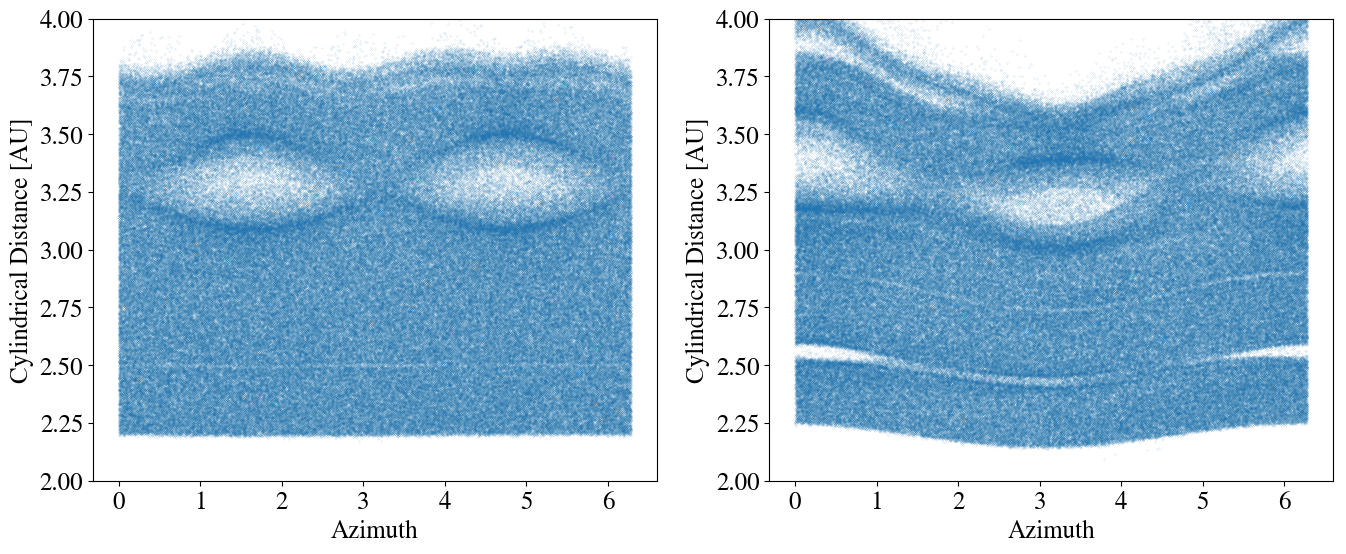
\includegraphics[width=\textwidth]{figures/rtheta.png}
    \caption{Caption goes here.\label{fig:rtheta}}
\end{figure*}

\begin{figure}
    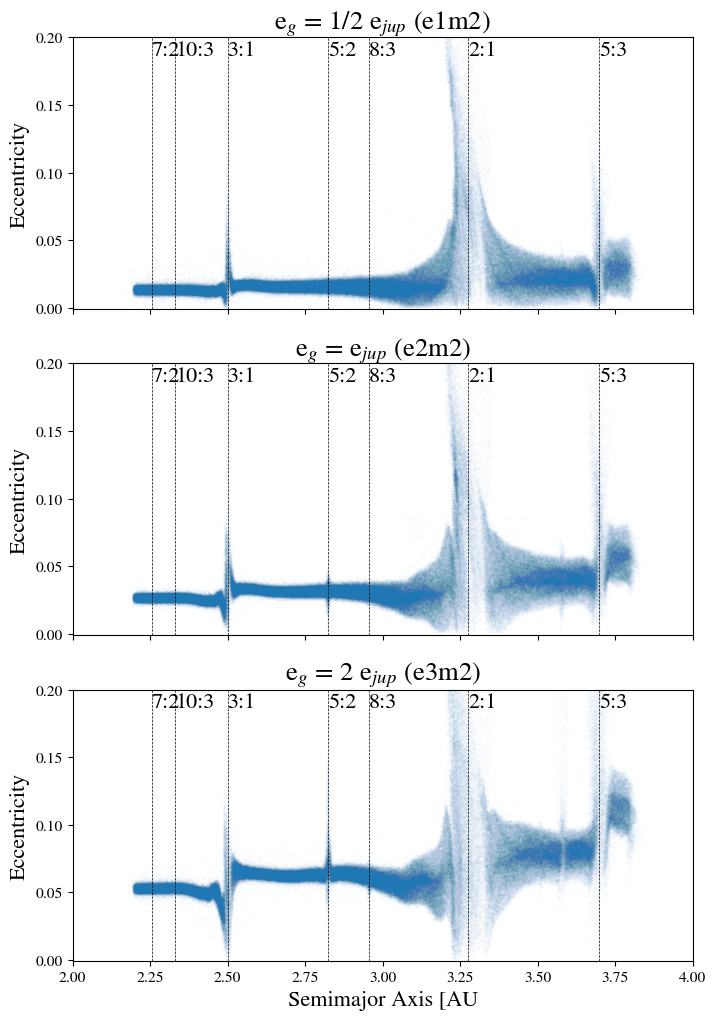
\includegraphics[width=\columnwidth]{figures/ae.png}
    \caption{Caption goes here.\label{fig:ae}}
\end{figure}

\begin{figure}
    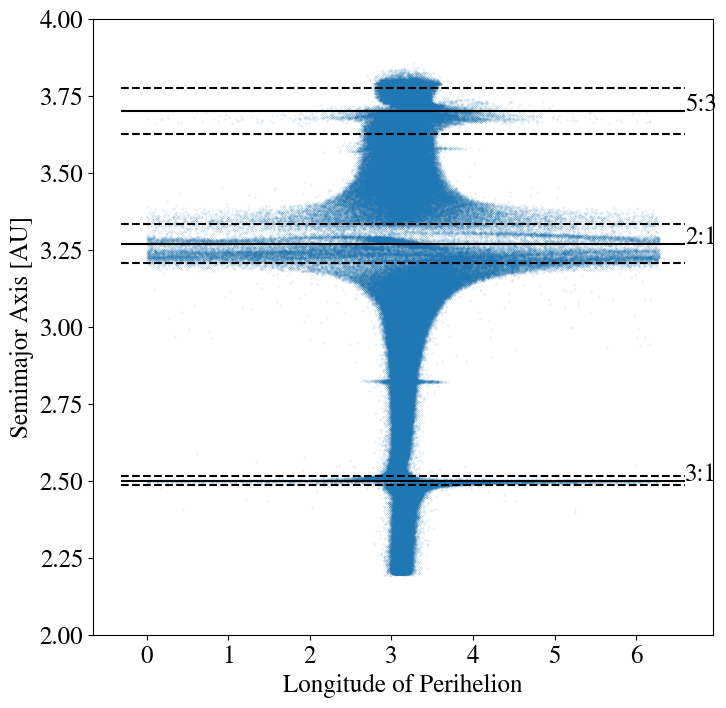
\includegraphics[width=\columnwidth]{figures/long_ph.png}
    \caption{Caption goes here.\label{fig:long_ph}}
\end{figure}

\begin{figure}
    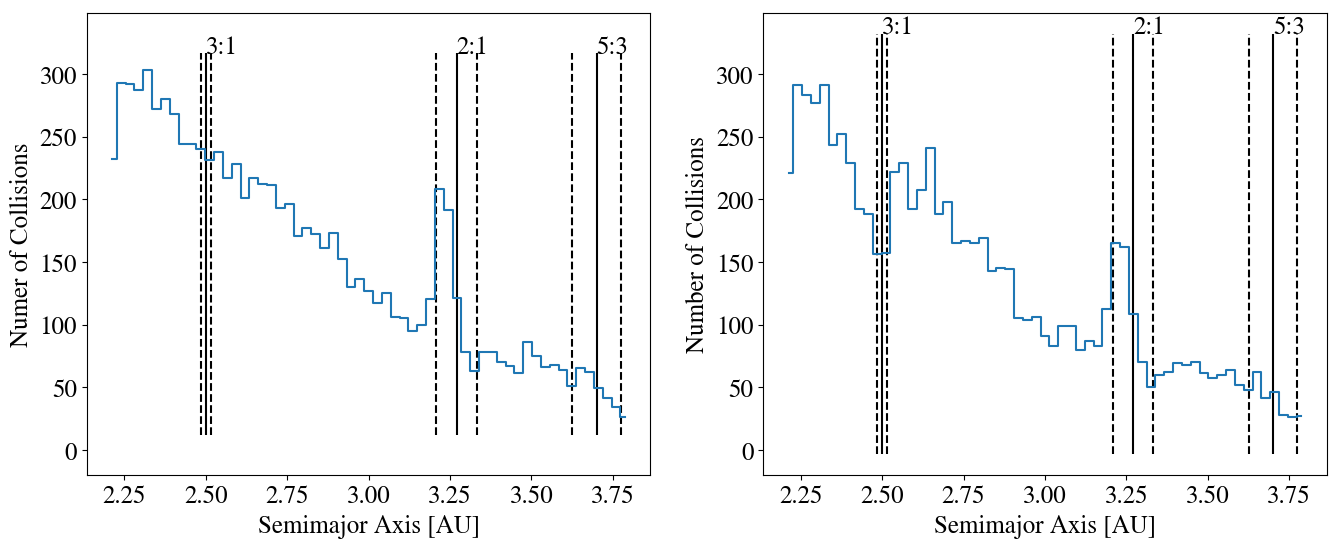
\includegraphics[width=\columnwidth]{figures/coll_hist_a.png}
    \caption{Caption goes here.\label{fig:coll_hist_a}}
\end{figure}

\begin{figure*}
    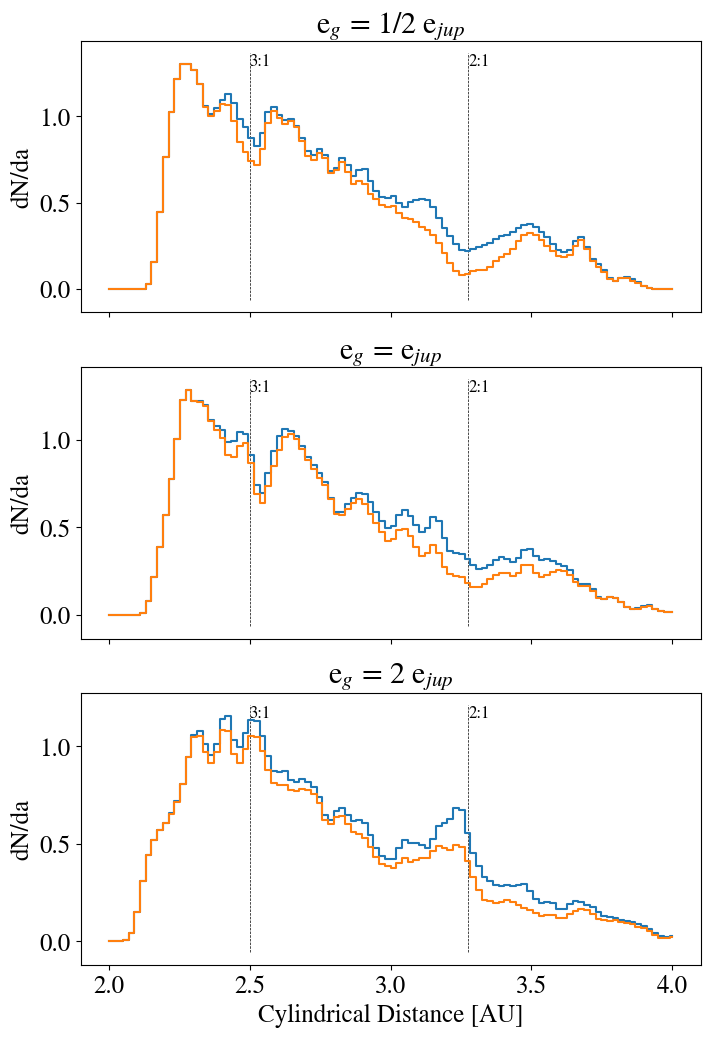
\includegraphics[width=\textwidth]{figures/coll_hist_r.png}
    \caption{Caption goes here.\label{fig:coll_hist_r}}
\end{figure*}

\section{Results} \label{sec:results}

We begin by examining the spatial distribution of planetesimals in both simulations. The polar position of the planetesimals at the 
end of the CJ and EJ simulations are shown in the left and right hand panels of  figure \ref{fig:rtheta}, respectively. Gaps produced by 
the 3:1, 2:1 and 5:3 MMR with Jupiter are visible in both cases. In the EJ case, a gap in the vicinity of the 5:2 MMR is also visible. 
The non-axisymmetric shape of the gaps reflects the fact that planetesimals in the vicinity of the resonances have been excited onto 
non-circular orbits. Although the spatial distribution of planetesimals near MMR in debris disks may provide clues to 
detect unseen planets, we will not focus on this topic here, as it has already been covered in detail by other studies 
\citep{2016ApJ...818..159T, 2018ApJ...857....3T}.

The MMRs are most clearly visible when viewing the semimajor axis and eccentricity distribution of the planetesimals. This is shown 
in figure \ref{fig:ae}. The top panel corresponds to the CJ simulation and the bottom panel corresponds to EJ. The solid vertical lines 
in this plot represent the nominal locations of the resonances. Near the nominal resonance locations, the a-e distribution of the 
planetesimals exhibits well-defined spikes which curve slightly inward due to conservation of the Jacobi energy. In the EJ simulation, 
the eccentricity distribution of bodies near resonance extends below the initial forced value. This is a reflection of the fact that these 
bodies are undergoing libration, which drives periodic oscillations in both semimajor axis and eccentricity. The coupling between 
these two quantities is described by equation \ref{eq:tiss}. In the EJ simulation, the eccentricity remains enhanced between the 
MMRs due to the secular forcing by Jupiter. This also has the consequence of making the eccentricity spikes more prominent. The 
reason for this is that the resonant perturbations scale with the eccentricity of the body in resonance $e$. This scaling is linear for a 
first order MMR, while the scaling is quadratic for a second order MMR. This results in a greater relative prominence of the features 
in figure \ref{fig:ae} of the 5:3 and 3:1 MMRs relative to the 2:1 in the EJ simulation.

The MMRs have one important additional effect, which is to drive precession of the longitude of perihelia of planetesimals near 
resonance. This effect becomes important in the EJ simulation, in which the orbits of bodies are initially aligned with that of Jupiter 
(see section \ref{sec:sec_force}). As is shown in figure \ref{fig:long_ph}, the strong precession induced by the MMRs overcomes the 
secular forcing and randomizes the orbital orientations of bodies near the resonances. The dashed horizontal lines in figure 
\ref{fig:long_ph} indicate the libration width of a planetesimal with an eccentricity of $e_{forced}$ at each resonance, which 
approximately shows the zone of influence of each MMR. When looking at the collision rates in the disk, this difference in the orbital 
orientations inside and outside of resonance will have an important effect on the radial structure of the second-generation dust, which 
will be discussed shortly.  Although this fast precession is also present in the CJ simulation, the longitude of perihelia of 
planetesimals in the disk exhibit no preferred direction, and so the precession from the MMRs produces no discernible difference in 
the orbital structure of the disk.

\subsection{Collision Rates}\label{sec:coll_rates}

The Safronov collision rate given by equation \ref{eq:safronov} can be a viable way to predict the collision rates of planetesimals 
using only their positions and velocities \citep{2017ApJ...850..103B}, but suffers from some limitations. First, the Safronov collision 
rate is constructed from the assumption that the planetesimal disk is azimuthally symmetric. This is not the case for the EJ 
simulation, in which the disk between resonances exhibits a well defined pericenter orientation. Although the strong precession 
induced by the MMRs does randomize the orientations of orbits near the resonances, the phase space distribution of bodies at the 
edges of the resonances becomes extremely complex and is best studied using a full N-body treatment. Secondly, as we will show 
below, the velocity distribution of planetesimals takes on a bimodal distribution near the MMRs. This makes the rms velocity of 
planetesimals not well-defined and therefore predicting the collision rate using a statistical approach becomes difficult.

Figure \ref{fig:coll_hist_a} shows the semimajor axis of collisions resolved in the CJ (top) and EJ simulations (bottom). The 
'semimajor axis of a collision' is defined as the semimajor axis of the first of the two planetesimals participating in a collision at the 
moment that it happens. To ensure that the definition of the first and second collider chosen by {\sc ChaNGa} does not influence 
these results, we also tried constructing figure \ref{fig:coll_hist_a} using the second collider and found no qualitative differences. 
Although both simulations were integrated and collisions were resolved for 5,000 years, we only show collisions that occurred during 
the last 3,000 years of the simulations. Before this time, the resonant features in the semimajor axis-eccentricity distribution (see 
figure \ref{fig:ae}) were still developing and had not yet reached a steady state. This results in transient features appearing in the 
collision profiles early on, which we exclude from figure \ref{fig:coll_hist_a} and all subsequent figures.

Most notably, the MMRs appear to have a measurable effect on the local collision rates. Slightly interior to the 2:1 resonance, the 
collision rate increases by a factor of roughly 2. In the EJ simulation, there is a significant deficiency in the number of collisions near 
the 3:1 MMR. We attribute this to the fact that the strength of a second order MMR scales as $e^{2}$, while a first order MMR scales 
linearly. Therefore, one would expect the 3:1 resonance to have more of an influence on the collision rate in a secularly perturbed 
disk. Although viewing the collision rate as a function of semimajor axis allows one to see a clear connection between the 
resonances and the collision rate, this does not immediately indicate where the dust generated by collisions will end up in the disk.

To construct a radial dust profile, we begin by making the assumption that any dust generated by collisions is strongly coupled to the 
gas. For a dust grain larger than the mean free path of the gas particles, the timescale to damp its eccentricity is given by 
\citep{1976PThPh..56.1756A}

\begin{equation}\label{eq:t_edamp}
    t_{e, damp} = \frac{8 s \rho}{3 e C_{D} \rho_{g} v_{th}}.
\end{equation}

where $m$, $e$ and $s$ are the mass, eccentricity and radius of the dust grain. $C_{D}$ is a drag coefficient which is of order unity, $
\rho_{g}$ is the local density of the gas and $v_{th}$ is its thermal speed. At 3 AU, the gaseous component of the solar nebula has a 
density of $4 \times 10^{-10}$ g cm$^{-3}$ and a typical thermal speed of $10^{5}$ cm s$^{-1}$ \citep{1981PThPS..70...35H}. For a 1 
mm dust grain with a density of 1 g cm$^{-3}$ and an eccentricity of 0.05, the damping timescale is $4 \times 10^{-3}$ years. This is 
orders of magnitude smaller than the collision timescale, therefore we expect that collisionally generated dust grains will immediately 
couple to the gas.

Operating under this assumption, a map of the relative concentration of second-generation dust can be constructed from simply the cylindrical distance at which the collisions occur. This is shown in the top panels of figure \ref{fig:coll_hist_r}, where the left side corresponds to the CJ simulation and the right side corresponds to EJ.

%Next, we move on to examine the statistics of the collisions that occur. Figure \ref{fig:coll_hist_a} shows the distribution of semimajor axes of every collision that is resolved. Here, the semimajor axis of a collision is defined as the semimajor axis of the first body participating in the collision at the moment that it occurs. During a collision, the determination of which body is first and which is second is determined by the collision search tree in {\sc ChaNGa}. To ensure that this does not introduce any bias, we also constructed figure \ref{fig:coll_hist_a} using the orbital parameters of the second body and found no qualitative difference. By examining the semimajor axis distribution of the collisions, it is easy to see how the MMRs affect the collision rates. The dashed lines again represent the libration width of each resonance and are meant to show its range of influence. In both the circular and eccentric Jupiter simulations, the collision rate is clearly enhanced interior to the 2:1 MMR. The 3:1 MMR only appears to have a noticeable influence on the collision rate in the EJ simulation. In both cases, although the 5:3 MMR has a clear influence on the on the semimajor-axis eccentricity distribution, it does not leave a measureable imprint on the collision rate. It is important to point out, however, that the libration width of sufficiently eccentric particles near the 5:3 MMR may extend beyond the outer edge of the disk and introduce boundary effects.

%Although the semimajor axis of a particle at the moment of collision provides useful information about how the mean motion resonances affect the collision rate in the disk, this information alone is not enough to predict where the second generation dust that is produced will end up. To do so, we will operate under the assumption that dust grains produced by collision events will quickly couple to the gas and attain a circular orbit. This assumption, which will be further justified in section \ref{sec:dust}, allows to map the radial variation in the dust surface density to the radial position of the collisions. This is shown in figure \ref{fig:coll_hist_r}, where the histograms indicate the x and y coordinates of a body at the moment that it undergoes a collision.

%Explanation of offset of feature near 3:1 in EJ: orbital orientations randomized near MMR, most bodies have ecc of e_forced, even in resonance. Geometrically, less overlap at apo, so surface density drops and so does coll rate.
Most notably, the prominent features visible in figure \ref{fig:coll_hist_a} adjacent to the 2:1 MMR no longer appear. This is due to the 
fact that the orbits of bodies in the 2:1 MMR have a wide range of eccentricities and therefore have the potential to undergo 
collisions at a wide range of heliocentric distances. In the CJ simulation, there is a prominent dip in the collision rate near the 2:1 
MMR. This feature is still moderately visible in the EJ simulation, but the dip is much wider and shallower. The random orientations of 
the orbits inside of the resonance (see figure \ref{fig:long_ph}), combined with the forced eccentricites of planetesimals adjacent to 
the resonance weakens the dip near the 2:1 MMR seen in the left hand panel of figure \ref{fig:coll_hist_a}. Additionally, there is a 
double-pronged feature in the collision rate near the 3:1 MMR in the EJ simulation. The radial distance of these two prongs 
corresponds to the maximum radial excursion that a planetesimal at the 3:1 MMR with an eccentricity set by secular forcing with 
Jupiter undergoes. (Need more explanation of why this happens)

As is seen in figure \ref{fig:long_ph}, the relatively fast precession rates induced by the mean motion resonances overpower the 
secular forcing by Jupiter and randomize the orientation of orbits near the nominal resonance locations. Of course, this difference in 
longitude of perihelion of bodies inside and outside of resonance is only present in the EJ simulation because the Jupiter imposes 
zero forced eccentricity on the disk when it has a circular orbit. Figure \ref{fig:m_hist} provides another view of the difference in 
collision statistics inside and outside and of resonance. This shows the mean anomalies of bodies at the moment that they undergo a 
collision. The top row corresponds to the EJ simulation and the bottom rom corresponds to the CJ simulation. The left panels 
correspond to collisions that occur inside of the 2:1 MMR and the right panels are for collisions that occur with a semimajor axis 
between 2.7 and 2.8 AU, which is meant to well away from the influence of any resonances. The semimajor axis window size in the 
right hand panel is chosen so that both histograms contain the same total number of collisions.

The qualitative differences between these four panels can be explained in the following way: for $\approx$ 100 km bodies, 
gravitational focusing plays a significant role in setting the collision rate. In regions of the disk where the rms eccentricity is small 
(which corresponds to a small velocity dispersion), the collision rate should be enhanced (see equation \ref{eq:safronov}). Inside of 
resonances, planetesimals undergo large amplitude libration which pumps up the eccentricity dispersion. This effect is visible in 
figure \ref{fig:ae} for both the EJ and CJ simulation. This implies that the collision rate should be geometric, and not depend on the 
velocity dispersion near resonances. When this is true, collisions should preferentially occur near perihelion. The reason for this is 
that in the geometric limit, the collision probability scales with the ratio between the geometric cross section of the two planetesimals 
and the surface area of a sphere with radius $r$, where $r$ is the distance between the bodies and the central star. This ratio, and 
therefore the collision probability, is largest when $r$ is minimized (see \citet{2003AJ....125.2692L}). The fact both of the left-hand 
panels in figure \ref{fig:m_hist} show a distinct lack of collisions near aphelion is consistent with this explanation.

Note that this trend is not present in the right-hand panels of figure \ref{fig:m_hist}. In the case with Jupiter on a circular orbit (bottom right panel), there is a spike in the collision rate both at perihelion and aphelion. The perihelion spike is still due to the geometric argument presented in the previous paragraph. The aphelion spike is due to the effect of gravitational focusing. At aphelion, bodies achieve their minimum speed. This lowers the relative velocity between planetesimals, which according to equation \ref{eq:safronov} should enhance the collision rate. Note that the collision rate does not exhibit much dependence on mean anomaly outside of resonance in the case with Jupiter on an eccentric orbit (top right panel). This is due to the secular forcing by Jupiter, which aligns the longitude of perihelia of adjacent planetesimals. The result of this is that bodies maintain similar relative speeds over the course of an orbit, even though the orbit is eccentric. This lack of variation in the relative speeds makes collisions equally likely at any orbital phase.

Motivate the assumption that dust produced in collisions immediately goes onto circular orbit

Discuss figure 5, hilight differences between surface density distribution and collision histogram. Calculation of safronov rate is hard because velocity distribution is bimodal in many places. Key features to point out: 2:1 MMR shows up well in CJ. Much more washed out in EJ, while 3:1 becomes more prominent. Also both features in EJ are shifted to the right of resonance location by a factor of (1+$e_{forced}$. This could be a viable way to measure ecc of the perturber.

\section{Observability of Collisions} \label{sec:dust}

Have aaron make a CASA dust emission map for the two histograms in figure 5. Fit a gaussian to the radial features and see if we can back out the eccentricity of the perturber and its mass. Also make 2d histogram showing how the perturbers eccentricity (which sets the forced eccentricity) and mass sets the libration width.

\section{Measuring Properties of the Perturber} \label{sec:fitting}

\section{Summary and Discussion} \label{sec:discuss}

\bibliography{references}

\clearpage

\end{document}
